\cleardoublepage

\section{实验与结果分析}

本章围绕本文提出的视频视觉 token 压缩方法进行实验验证与结果分析。实验主要从压缩效率、模型准确率、不同压缩倍率下的鲁棒性以及跨数据集泛化能力等方面展开。本文以 VideoLLaMA2-7B-16F 作为基础视频大模型，在不改变语言模型、视觉塔和原始时空连接模块主体结构的前提下，将 TokenPacker 作为帧级空间视觉 token 压缩模块接入模型推理流程，并在 MVBench 数据集上进行主要实验验证\cite{videollama22024,mvbench2024,tokenpacker2024}。

本章实验重点回答以下问题：第一，引入视觉 token 压缩后，模型的视觉 token 数量、推理延迟与吞吐率是否得到改善；第二，TokenPacker 直接迁移到 VideoLLaMA2 后是否存在性能下降问题，token 校准与轻量微调能否缓解该问题；第三，在不同压缩倍率下，本文方法与 Mean Pooling 等固定压缩方法相比是否具有更好的高压缩鲁棒性；第四，在不使用目标测试集进行校准的情况下，本文方法是否具备一定跨数据集泛化能力。

\subsection{实验环境与数据集}

\subsubsection{实验环境}

\begin{table}[htbp]
    \centering
    \caption{\label{tab:experiment_environment}实验软硬件环境}
    \begin{tabularx}{\textwidth}{lX}
        \toprule
        类型 & 配置 \\
        \midrule
        GPU & NVIDIA GeForce RTX 4090 \\
        显存 & 24 GB \\
        GPU Driver & 580.105.08 \\
        NVIDIA-SMI CUDA Version & 13.0 \\
        PyTorch & 2.2.0+cu118 \\
        PyTorch CUDA Runtime & 11.8 \\
        Transformers & 4.40.0 \\
        Python 环境 & Miniconda, Python 3.12 \\
        \bottomrule
    \end{tabularx}
\end{table}

本文实验在单卡 NVIDIA GeForce RTX 4090 平台上完成。训练与推理均采用 batch size 为 1 的设置，并在相同硬件环境下统计模型推理延迟、prefill 时间、decode 时间、吞吐率与峰值显存。实验所使用的主要软硬件环境如\autoref{tab:experiment_environment}所示。

需要说明的是，NVIDIA-SMI 中显示的 CUDA Version 表示驱动支持的最高 CUDA 版本，而本文 PyTorch 实际运行时使用的是 CUDA 11.8。为保证不同方法之间的对比公平性，所有推理实验均在相同硬件环境、相同 batch size 和相同解码设置下完成。

\subsubsection{基础模型与视觉配置}

本文采用 DAMO-NLP-SG/VideoLLaMA2-7B-16F 作为基础模型。该模型使用 CLIP 视觉塔进行逐帧视觉特征提取，视觉输入分辨率为 $336\times336$，patch 网格大小为 $24\times24$，因此单帧原始空间视觉 token 数量为 576。实验统一使用 16 帧视频输入，因此在不进行压缩时，每个视频样本对应的帧级空间视觉 token 总数为：

\begin{equation}
    \label{equ:raw_video_token_number_exp}
    N_{\mathrm{raw}} = 16 \times 576 = 9216
\end{equation}

压缩模块插入在视觉塔输出与后续时序聚合/投影模块之间，对每一帧内部的空间视觉 token 进行压缩。除特别说明外，语言模型、视觉塔和原始 projector 均保持冻结，仅训练 TokenPacker core。基础视觉配置如\autoref{tab:basic_model_config}所示。

\begin{table}[htbp]
    \centering
    \caption{\label{tab:basic_model_config}基础模型与视觉输入配置}
    \begin{tabularx}{\textwidth}{lX}
        \toprule
        项目 & 设置 \\
        \midrule
        基础模型 & DAMO-NLP-SG/VideoLLaMA2-7B-16F \\
        视觉塔 & openai/clip-vit-large-patch14-336 \\
        输入帧数 & 16 \\
        原始空间网格 & $24\times24$ \\
        原始 token 数 & 576 tokens/frame \\
        解码设置 & greedy decoding, do\_sample=False \\
        随机种子 & 42 \\
        \bottomrule
    \end{tabularx}
\end{table}

\subsubsection{数据集设置}

本文主要使用 MVBench 作为主实验数据集。MVBench 是面向视频多模态理解任务的综合评测基准，包含动作识别、动作预测、物体交互、场景变化、时序推理等多个子任务，能够较全面地评估视频大模型的时空理解能力\cite{mvbench2024}。在本文实验中，MVBench 同时用于构造无标签 token 校准数据和正式下游评测数据。为避免训练与测试重叠，本文从 MVBench 中构造校准子集，并在正式评测时显式排除该子集。

具体而言，校准子集从 MVBench 的 20 个任务类别中分别随机抽取最多 50 个视频，形成 `data/calibration\_videos\_mvbench\_clip.txt`。该文件仅用于阶段一无标签 token 校准和可选的阶段二轻量监督微调。正式 MVBench 评测时使用 `--exclude-video-list` 参数排除该校准子集，并在每个任务类别中最多抽取 50 个视频用于评测。该设置能够降低校准数据泄漏对评测结果的影响。

此外，本文使用 Video-MME 作为跨数据集泛化测试集\cite{videomme2025}。Video-MME 不参与 TokenPacker 的校准或监督微调，仅用于测试 MVBench 上获得的压缩模型在新数据集上的泛化能力。与 MVBench 相比，Video-MME 覆盖感知、识别、推理和信息概括等更多类型的视频理解任务，因此能够用于观察压缩模块是否只适配 MVBench 分布，或是否能够迁移到新的评测基准上。

\subsubsection{对比方法}

本文比较的主要方法包括未压缩 Baseline、Mean Pooling、TokenPacker Init、TokenPacker Calibrated 和 TokenPacker Finetuned。所有压缩方法均在相同 scale factor 下进行对比，以保证每帧视觉 token 预算一致。各方法说明如\autoref{tab:comparison_methods}所示。

\begin{table}[htbp]
    \centering
    \caption{\label{tab:comparison_methods}实验对比方法}
    \begin{tabularx}{\textwidth}{lX}
        \toprule
        方法 & 说明 \\
        \midrule
        Baseline & 不进行视觉 token 压缩，保留每帧 576 个空间 token \\
        Mean Pooling & 使用非重叠均值池化压缩每帧空间 token \\
        TokenPacker Init & 使用官方 TokenPacker 权重迁移得到的 core checkpoint \\
        TokenPacker Calibrated & 在 MVBench 校准子集上进行无标签 token 校准后的 TokenPacker \\
        TokenPacker Finetuned & 在校准 checkpoint 基础上继续进行轻量监督微调后的 TokenPacker \\
        \bottomrule
    \end{tabularx}
\end{table}

其中，Mean Pooling 是一种固定压缩方法，不引入额外可学习参数，直接对相邻空间 token 进行均值聚合。TokenPacker 则属于可学习视觉 token 压缩方法，其通过注意力机制将高分辨率局部视觉信息聚合到低分辨率 query token 中。二者的对比能够反映“分布保持型固定压缩方法”和“可学习 token 聚合方法”在不同压缩倍率下的性能差异。

\subsubsection{压缩比例与评价指标}

由于 CLIP 视觉塔的空间网格为 $24\times24$，本文设置的 scale factor 分别为 2、3 和 4，均可整除原始空间网格，因此无需额外 padding。不同压缩倍率对应的每帧 token 数如\autoref{tab:compression_scale_setting}所示。

\begin{table}[htbp]
    \centering
    \caption{\label{tab:compression_scale_setting}不同压缩倍率下的 token 预算}
    \begin{tabularx}{\textwidth}{c c c X}
        \toprule
        Scale Factor & 每帧 token 数 & 相对原始 token 比例 & 说明 \\
        \midrule
        1 & 576 & 100.00\% & Baseline，无压缩 \\
        2 & 144 & 25.00\% & 中等压缩率 \\
        3 & 64 & 11.11\% & 高压缩率 \\
        4 & 36 & 6.25\% & 极高压缩率 \\
        \bottomrule
    \end{tabularx}
\end{table}

本文主要采用以下指标评价模型表现：Accuracy 用于衡量视频问答任务准确率；Avg Compressed Tokens 用于衡量压缩后的平均视觉 token 数量；Compression Ratio 用于衡量压缩后 token 数量相对于原始 token 数量的比例；Avg Latency 用于衡量单样本平均推理延迟；Prefill Time 用于衡量输入上下文处理阶段耗时；Decode Time 用于衡量答案生成阶段耗时；Throughput 用于衡量单位时间内可处理样本数量；Peak Memory 用于衡量推理过程中的峰值显存占用。

\subsection{压缩效率实验}

本节主要验证本文方法是否能够有效降低视觉 token 数量并提升推理效率。实验在 MVBench 正式评测集上进行，对比未压缩 Baseline 与 TokenPacker 在 scale factor 分别为 2、3、4 时的效率表现。实验结果如\autoref{tab:compression_efficiency_result}所示。

\begin{table}[htbp]
    \centering
    \small
    \caption{\label{tab:compression_efficiency_result}压缩效率实验结果}
    \resizebox{\textwidth}{!}{
    \begin{tabular}{l c c c c c c c c}
        \toprule
        Method & Scale & Compression Ratio & Accuracy & Avg Tokens & Avg Latency(s) & Prefill(s) & Decode(s) & Throughput \\
        \midrule
        Baseline & None & 1.0000 & 57.37\% & 9216 & 0.4762 & 0.1943 & 0.1597 & 2.1000 \\
        TokenPacker & 2 & 0.2500 & 41.32\% & 2304 & 0.3699 & 0.0775 & 0.1852 & 2.7037 \\
        TokenPacker & 3 & 0.1111 & 37.41\% & 1024 & 0.3431 & 0.0539 & 0.1881 & 2.9143 \\
        TokenPacker & 4 & 0.0625 & 36.66\% & 576 & 0.3344 & 0.0443 & 0.1896 & 2.9900 \\
        \bottomrule
    \end{tabular}}
\end{table}

从 token 数量来看，未压缩 Baseline 的平均视觉 token 数量为 9216。当 scale factor 为 2 时，压缩后 token 数量下降到 2304，相当于原始 token 数量的 25.00\%；当 scale factor 为 3 时，压缩后 token 数量进一步下降到 1024，相当于原始 token 数量的 11.11\%；当 scale factor 为 4 时，压缩后 token 数量下降到 576，仅为原始 token 数量的 6.25\%。这说明本文接入的帧级空间 token 压缩模块能够按照预设压缩倍率有效降低视频视觉 token 数量。

从推理延迟来看，Baseline 的平均推理延迟为 0.4762 秒。TokenPacker 在 scale factor 为 2、3、4 时的平均推理延迟分别为 0.3699 秒、0.3431 秒和 0.3344 秒。与 Baseline 相比，三种压缩设置分别带来了 22.3\%、28.0\% 和 29.8\% 的延迟下降。与此同时，吞吐率从 Baseline 的 2.1000 samples/s 分别提升到 2.7037、2.9143 和 2.9900 samples/s，对应吞吐率增益分别为 28.7\%、38.8\% 和 42.4\%。效率提升结果如\autoref{tab:efficiency_gain_result}所示。

\begin{table}[htbp]
    \centering
    \caption{\label{tab:efficiency_gain_result}不同压缩倍率下的效率收益}
    \begin{tabular}{c c c c}
        \toprule
        Scale & Accuracy Drop & Latency Reduction & Throughput Gain \\
        \midrule
        2 & -16.05\% & 22.3\% & 28.7\% \\
        3 & -19.96\% & 28.0\% & 38.8\% \\
        4 & -20.71\% & 29.8\% & 42.4\% \\
        \bottomrule
    \end{tabular}
\end{table}

进一步分析 prefill 与 decode 阶段可以发现，视觉 token 压缩主要降低的是 prefill 阶段耗时。Baseline 的 prefill 时间为 0.1943 秒，而 scale factor 为 2、3、4 时分别下降到 0.0775 秒、0.0539 秒和 0.0443 秒。这一现象符合视频多模态大模型的推理过程特点：视觉 token 主要作为输入上下文参与 prefill 阶段计算，减少视觉 token 数量能够直接降低上下文编码阶段的注意力计算开销。相比之下，decode 阶段耗时变化并不明显，甚至略有增加，说明本文方法的主要效率收益来自视觉上下文长度的压缩，而不是答案生成阶段本身的加速。

从准确率角度看，压缩带来了不同程度的性能下降。Baseline 准确率为 57.37\%，TokenPacker 在 scale factor 为 2、3、4 时准确率分别为 41.32\%、37.41\% 和 36.66\%。这说明视觉 token 压缩虽然能够显著降低推理开销，但也会造成一定视觉信息损失和模型适配问题。因此，后续实验需要进一步分析 TokenPacker 直接迁移、token 校准和轻量微调对模型准确率的影响。

\subsection{模型性能对比实验}

本节比较不同方法在 MVBench 上的准确率表现，重点分析 TokenPacker 直接迁移到 VideoLLaMA2 后的性能变化，以及 token 校准和轻量监督微调对性能恢复的作用。实验主要以 scale factor 为 2 的设置进行详细分析，同时在后续小节中进一步比较不同压缩倍率下的变化趋势。

\subsubsection{Scale Factor 为 2 时的整体性能对比}

在 scale factor 为 2 的设置下，不同方法的整体准确率如\autoref{tab:s2_overall_performance}所示。

\begin{table}[htbp]
    \centering
    \caption{\label{tab:s2_overall_performance}Scale factor 为 2 时的整体准确率对比}
    \begin{tabular}{l c}
        \toprule
        Method & Overall Accuracy \\
        \midrule
        VideoLLaMA2 Baseline & 57.37 \\
        Mean Pooling (s2) & 50.47 \\
        TokenPacker (s2) & 33.86 \\
        TokenPacker + Calibration (s2) & 41.32 \\
        TokenPacker + Finetune (s2) & 47.01 \\
        \bottomrule
    \end{tabular}
\end{table}

可以看到，未压缩 VideoLLaMA2 Baseline 的准确率最高，为 57.37\%。Mean Pooling 在压缩到每帧 144 个 token 后，准确率为 50.47\%，相比 Baseline 下降 6.90 个百分点。TokenPacker 直接迁移后的准确率仅为 33.86\%，相比 Baseline 下降 23.51 个百分点，说明原始 TokenPacker 权重虽然能够完成视觉 token 压缩，但直接迁移到 VideoLLaMA2 的视频推理流程中存在明显适配问题。

经过无标签 token 校准后，TokenPacker 准确率从 33.86\% 提升到 41.32\%，提升 7.46 个百分点。进一步进行轻量监督微调后，准确率提升到 47.01\%，相比直接迁移版本提升 13.15 个百分点，相比校准版本进一步提升 5.69 个百分点。这说明 token 校准和轻量微调均能够缓解 TokenPacker 迁移后的性能下降问题。

\begin{figure}[htbp]
    \centering
    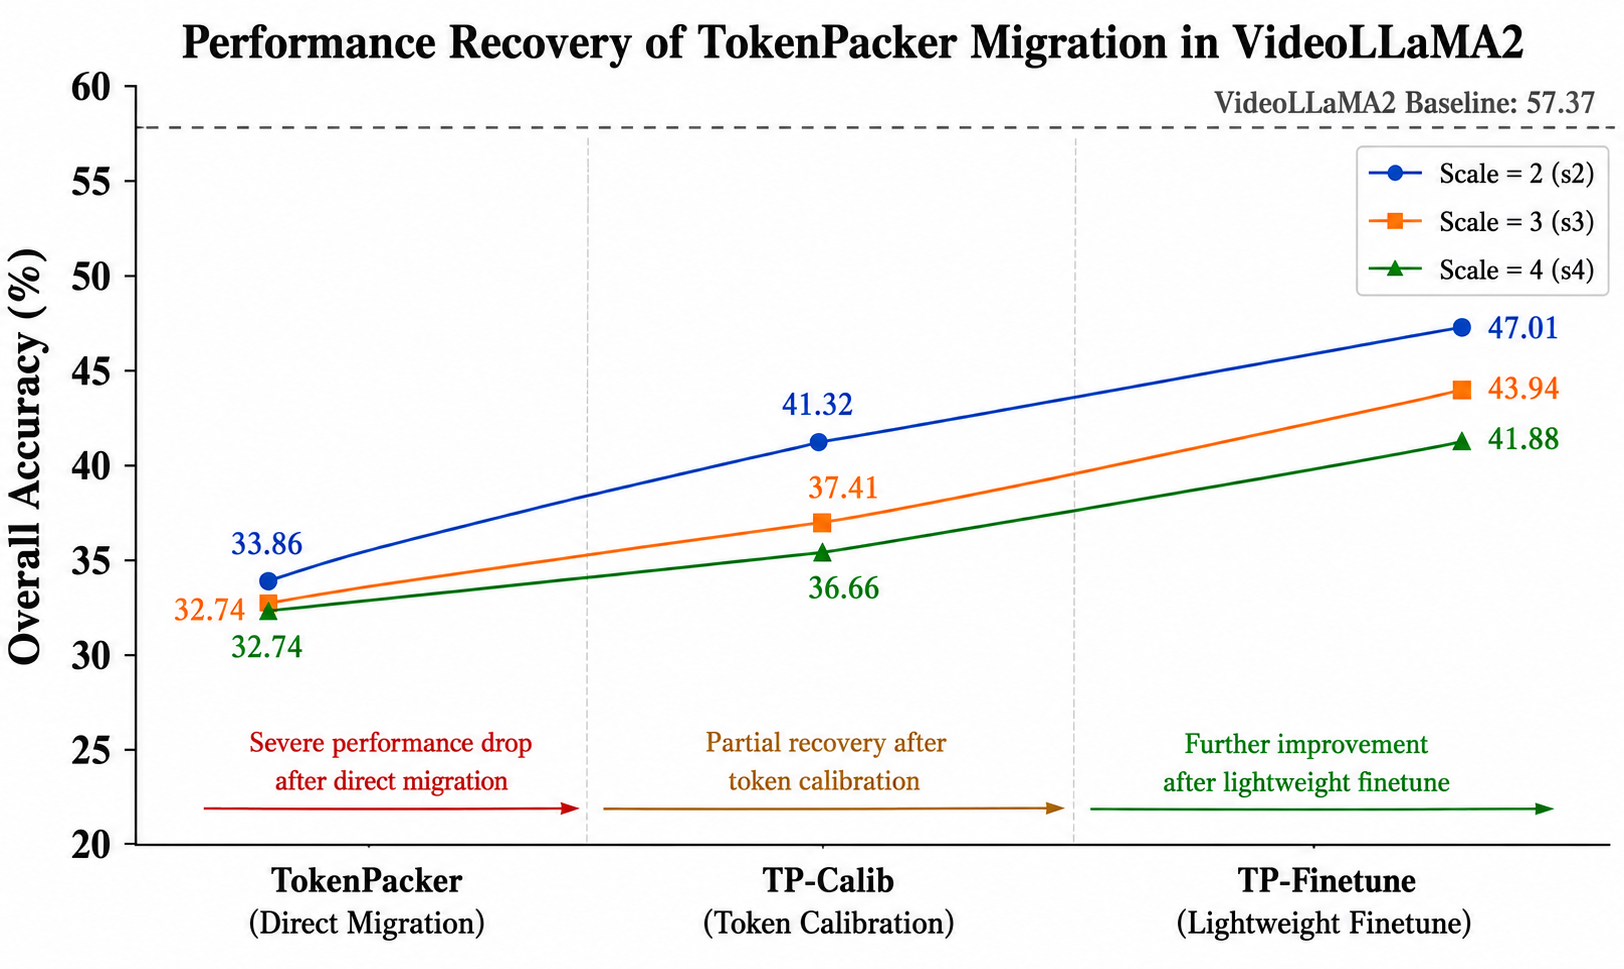
\includegraphics[width=0.88\textwidth]{figure/experiment/exp_img2.png}
    \caption{\label{fig:performance_recovery}TokenPacker 迁移到 VideoLLaMA2 后的性能恢复过程}
\end{figure}

\autoref{fig:performance_recovery}展示了 TokenPacker 从直接迁移到校准、再到轻量微调的性能恢复过程。可以看到，直接迁移阶段模型准确率下降较为明显，说明图像场景下训练得到的 TokenPacker 并不能直接与 VideoLLaMA2 的视觉特征分布和 STC Connector 输入要求完全匹配。经过 token 校准后，模型准确率得到初步恢复，说明无标签特征分布对齐能够改善压缩 token 与原始视觉 token 之间的表示差异。进一步微调后，模型性能继续提升，表明在下游任务监督信号的约束下，TokenPacker 能够学习到更适合视频问答任务的压缩表示。

\subsubsection{Scale Factor 为 2 时的子任务性能}

为了进一步分析不同方法在各类视频理解能力上的表现，本文统计了 scale factor 为 2 时各方法在 MVBench 不同子任务上的准确率，结果如\autoref{tab:s2_category_performance}所示。

\begin{table}[htbp]
    \centering
    \scriptsize
    \caption{\label{tab:s2_category_performance}Scale factor 为 2 时不同子任务准确率对比}
    \resizebox{\textwidth}{!}{
    \begin{tabular}{l c c c c c}
        \toprule
        Category & Baseline & Mean Pooling & TokenPacker & TP + Calibration & TP + Finetune \\
        \midrule
        Action Sequence & 75.61 & 64.63 & 25.61 & 39.02 & 48.78 \\
        Action Prediction & 55.71 & 44.29 & 34.29 & 44.29 & 50.00 \\
        Action Antonym & 88.00 & 74.00 & 16.00 & 46.00 & 60.00 \\
        Fine-grained Action & 60.00 & 56.00 & 22.00 & 30.00 & 46.00 \\
        Unexpected Action & 66.07 & 64.29 & 32.14 & 35.71 & 57.14 \\
        Object Existence & 62.50 & 50.00 & 42.86 & 51.79 & 48.21 \\
        Object Interaction & 68.75 & 59.38 & 25.00 & 40.63 & 62.50 \\
        Object Shuffle & 38.00 & 30.00 & 30.00 & 34.00 & 26.00 \\
        Moving Direction & 24.53 & 18.87 & 35.85 & 24.53 & 22.64 \\
        Action Localization & 42.00 & 34.00 & 34.00 & 26.00 & 32.00 \\
        Scene Transition & 90.00 & 80.00 & 44.00 & 78.00 & 70.00 \\
        Action Count & 48.00 & 44.00 & 44.00 & 46.00 & 44.00 \\
        Moving Count & 57.41 & 59.26 & 42.59 & 51.85 & 61.11 \\
        Moving Attribute & 55.36 & 53.57 & 30.36 & 42.86 & 50.00 \\
        State Change & 51.92 & 46.15 & 46.15 & 38.46 & 48.08 \\
        Character Order & 57.41 & 38.89 & 38.89 & 35.19 & 44.44 \\
        Egocentric Navigation & 40.00 & 42.00 & 34.00 & 38.00 & 36.00 \\
        Episodic Reasoning & 58.46 & 56.92 & 41.54 & 44.62 & 46.15 \\
        Counterfactual Inference & 40.00 & 35.00 & 28.33 & 38.33 & 35.00 \\
        \midrule
        Overall & 57.37 & 50.47 & 33.86 & 41.32 & 47.01 \\
        \bottomrule
    \end{tabular}}
\end{table}

从子任务结果可以看出，TokenPacker 直接迁移在多数任务上均出现明显下降，尤其是在 Action Antonym、Fine-grained Action、Object Interaction 和 Scene Transition 等任务上下降较大。这些任务通常要求模型准确保留局部视觉语义、动作状态变化或场景转移信息，因此对视觉 token 的表达质量较为敏感。直接迁移的 TokenPacker 由于未充分适配 VideoLLaMA2 的视觉特征分布，压缩后的 token 难以稳定保留这些细粒度信息。

经过 token 校准后，多数子任务准确率得到恢复。例如，Action Antonym 从 16.00\% 提升到 46.00\%，Scene Transition 从 44.00\% 提升到 78.00\%，Object Interaction 从 25.00\% 提升到 40.63\%。这说明无标签校准能够在一定程度上缓解压缩 token 与原始模型视觉表示之间的分布偏移问题。

轻量微调进一步改善了部分任务表现。例如，Object Interaction 提升到 62.50\%，Moving Count 提升到 61.11\%，Action Prediction 提升到 50.00\%。这些结果表明，监督微调能够进一步利用下游任务信号，使 TokenPacker 学习到更适合视频问答任务的视觉压缩表示。然而，也有部分任务如 Object Shuffle、Egocentric Navigation 和 Counterfactual Inference 的提升并不稳定，说明当前轻量微调规模有限，仍不足以全面恢复所有类型的视频推理能力。

\subsubsection{Token 校准与轻量微调的增益分析}

为了更清晰地观察校准和微调带来的性能变化，本文统计了不同 scale factor 下 TokenPacker 直接迁移、校准和微调后的整体准确率变化。校准增益如\autoref{tab:calibration_gain}所示。

\begin{table}[htbp]
    \centering
    \caption{\label{tab:calibration_gain}Token 校准带来的准确率增益}
    \begin{tabular}{c c c c}
        \toprule
        Scale & TokenPacker & TP-Calib & Gain \\
        \midrule
        2 & 33.86 & 41.32 & +7.46 \\
        3 & 32.74 & 37.41 & +4.67 \\
        4 & 32.74 & 36.66 & +3.92 \\
        \bottomrule
    \end{tabular}
\end{table}

结果表明，token 校准在三个压缩倍率下均带来了准确率提升。其中，scale factor 为 2 时提升最明显，准确率提升 7.46 个百分点；scale factor 为 3 和 4 时分别提升 4.67 和 3.92 个百分点。这一现象说明，当压缩倍率较低、保留 token 数量相对较多时，TokenPacker 仍有较充分的信息容量用于对齐原始视觉 token 分布，因此校准带来的收益更明显。而在更高压缩倍率下，由于 token 预算更小，视觉信息本身已经被更强地压缩，校准能够恢复的性能空间相对有限。

轻量监督微调的增益如\autoref{tab:finetune_gain}所示。

\begin{table}[htbp]
    \centering
    \caption{\label{tab:finetune_gain}轻量监督微调带来的准确率增益}
    \begin{tabular}{c c c c}
        \toprule
        Scale & TP-Calib & TP-Finetune & Gain \\
        \midrule
        2 & 41.32 & 47.01 & +5.69 \\
        3 & 37.41 & 43.94 & +6.53 \\
        4 & 36.66 & 41.88 & +5.22 \\
        \bottomrule
    \end{tabular}
\end{table}

可以看到，轻量微调在三个压缩倍率下同样均带来进一步提升。其中，scale factor 为 3 时提升 6.53 个百分点，scale factor 为 4 时提升 5.22 个百分点，说明在高压缩设置下，任务监督信号对压缩 token 表示的优化仍然有效。与 token 校准相比，轻量微调不仅关注压缩 token 与原始视觉 token 的特征一致性，还直接优化下游问答任务表现，因此能够在校准基础上进一步恢复准确率。

总体而言，TokenPacker 直接迁移存在明显的分布适配问题；无标签 token 校准能够缓解视觉 token 分布偏移；轻量监督微调则进一步增强压缩模块对下游任务的适配能力。这一结果说明，本文方法不是简单地插入一个图像 token 压缩模块，而是需要结合视频大模型的视觉特征结构进行迁移、校准和任务适配。

\subsection{不同压缩倍率下的鲁棒性实验}

本节进一步分析不同压缩倍率下各方法的准确率变化趋势，重点比较 Mean Pooling 与 TokenPacker 系列方法在高压缩倍率下的鲁棒性。实验设置 scale factor 分别为 2、3 和 4，对应每帧 token 数分别为 144、64 和 36。

\subsubsection{不同压缩倍率下的整体准确率}

不同方法在不同压缩倍率下的整体准确率如\autoref{tab:scale_overall_accuracy}所示。

\begin{table}[htbp]
    \centering
    \caption{\label{tab:scale_overall_accuracy}不同压缩倍率下的整体准确率对比}
    \begin{tabular}{c c c c c}
        \toprule
        Scale & Mean Pooling & TokenPacker & TP-Calib & TP-Finetune \\
        \midrule
        2 & 50.47 & 33.86 & 41.32 & 47.01 \\
        3 & 43.66 & 32.74 & 37.41 & 43.94 \\
        4 & 39.37 & 32.74 & 36.66 & 41.88 \\
        \bottomrule
    \end{tabular}
\end{table}

\begin{figure}[htbp]
    \centering
    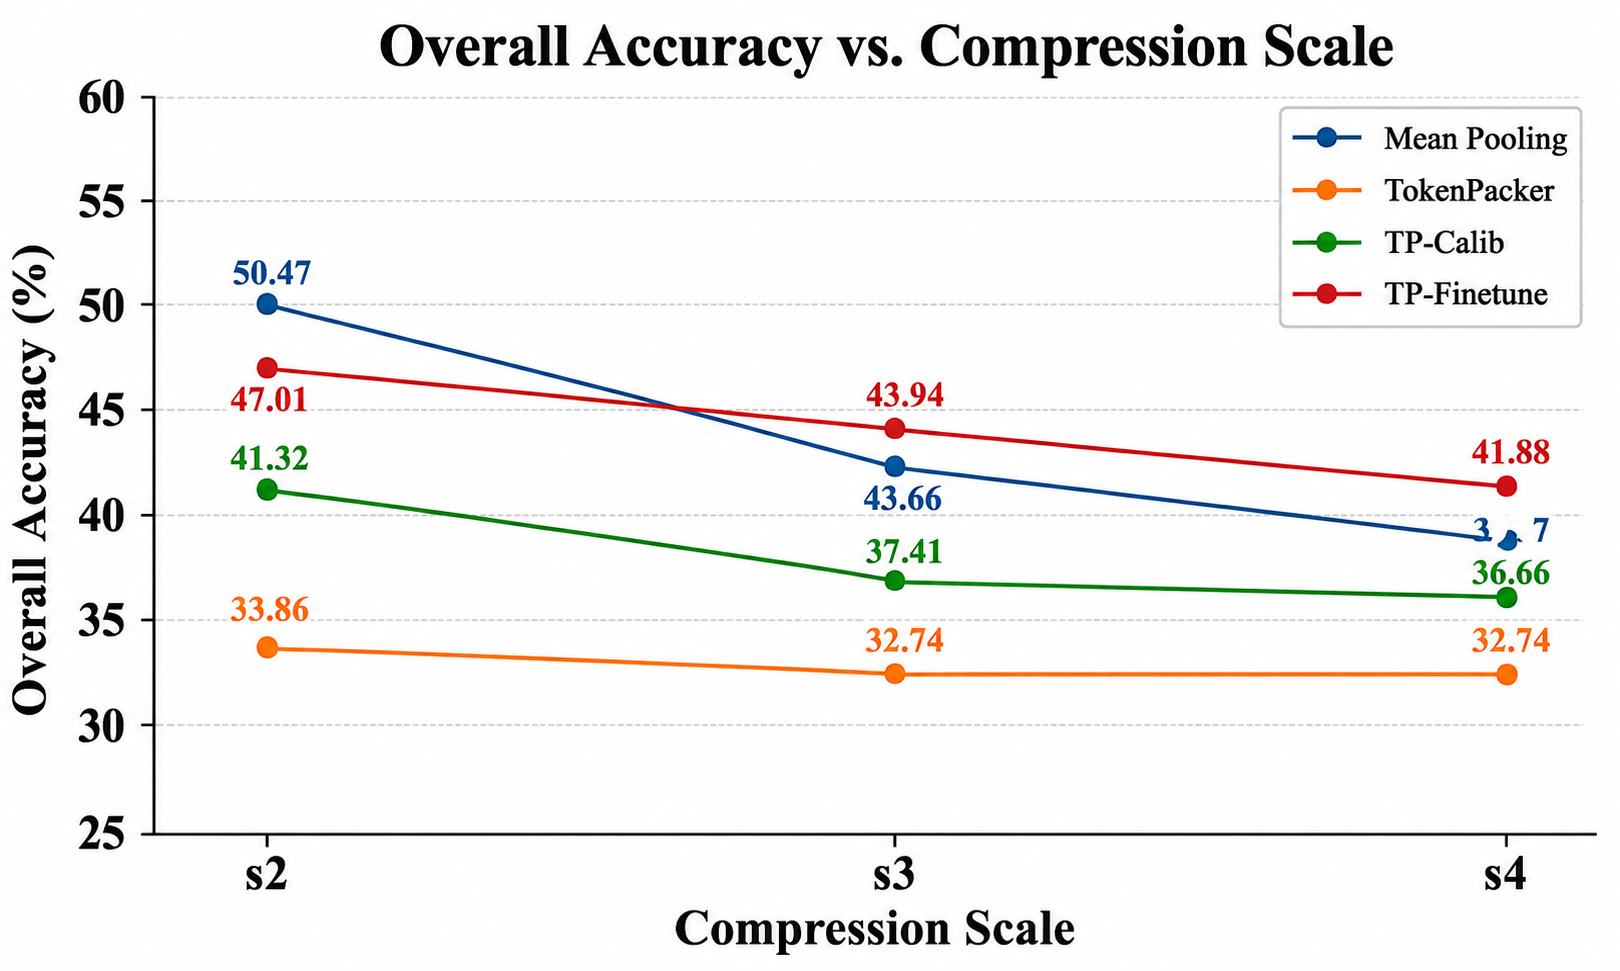
\includegraphics[width=0.88\textwidth]{figure/experiment/exp_img1.png}
    \caption{\label{fig:overall_accuracy_vs_scale}不同压缩倍率下整体准确率变化趋势}
\end{figure}

\autoref{fig:overall_accuracy_vs_scale}展示了不同压缩倍率下各方法整体准确率的变化趋势。可以看到，Mean Pooling 在 scale factor 为 2 时取得了较高准确率，达到 50.47\%，明显高于 TokenPacker 直接迁移和校准后的结果。这说明在较低压缩倍率下，简单均值池化能够较好地保持原始视觉 token 的分布形态，与 VideoLLaMA2 原始后端模块具有较好的适配性。

然而，随着压缩倍率提高，Mean Pooling 的准确率下降较为明显。当 scale factor 从 2 增加到 4 时，Mean Pooling 准确率从 50.47\% 下降到 39.37\%，下降 11.10 个百分点。这说明固定均值池化方法对高压缩倍率较为敏感。当每帧 token 数量从 144 进一步压缩到 36 时，简单平均操作难以保留足够的局部视觉细节和细粒度语义信息。

相比之下，TokenPacker 系列方法在不同 scale factor 下的下降趋势更平缓。TokenPacker 直接迁移版本从 scale factor 为 2 到 4 仅下降 1.12 个百分点；TokenPacker + Calibration 下降 4.66 个百分点；TokenPacker + Finetune 下降 5.13 个百分点。虽然 TokenPacker 在低压缩倍率下仍低于 Mean Pooling，但在高压缩倍率下差距逐渐缩小。特别是在 scale factor 为 4 时，TokenPacker + Finetune 的准确率达到 41.88\%，超过 Mean Pooling 的 39.37\%。这一结果说明，可学习 token 压缩方法在极高压缩率下具有更好的信息聚合能力和压缩鲁棒性。

\subsubsection{准确率下降趋势分析}

为进一步量化不同方法对压缩倍率变化的敏感性，本文统计了 scale factor 从 2 增加到 4 时各方法的准确率变化，结果如\autoref{tab:accuracy_drop_scale}所示。

\begin{table}[htbp]
    \centering
    \caption{\label{tab:accuracy_drop_scale}不同方法随压缩倍率增加的准确率变化}
    \begin{tabular}{l c c c c}
        \toprule
        Method & Scale=2 & Scale=3 & Scale=4 & $\Delta$(s2$\rightarrow$s4) \\
        \midrule
        Mean Pooling & 50.47 & 43.66 & 39.37 & -11.10 \\
        TokenPacker & 33.86 & 32.74 & 32.74 & -1.12 \\
        TP + Calibration & 41.32 & 37.41 & 36.66 & -4.66 \\
        TP + Finetune & 47.01 & 43.94 & 41.88 & -5.13 \\
        \bottomrule
    \end{tabular}
\end{table}

从下降幅度看，Mean Pooling 的准确率下降最大，说明其在高压缩倍率下难以稳定保持任务性能。其原因在于 Mean Pooling 直接对局部 token 求平均，虽然能够较好保留整体分布形态，但缺乏对局部重要区域的自适应选择能力。当压缩倍率较高时，大量细粒度视觉信息被平均化，容易削弱模型对动作细节、目标交互和场景变化的判断能力。

TokenPacker 直接迁移版本的下降幅度最小，但其整体准确率较低。这说明原始 TokenPacker 在不同压缩倍率下具有一定结构稳定性，但由于其未充分适配 VideoLLaMA2 的视觉特征分布和 STC Connector 输入要求，导致整体性能处于较低水平。经过校准和微调后，TokenPacker 的整体准确率明显提升，同时仍保持相对平缓的下降趋势。这表明 TokenPacker 的注意力聚合机制在高压缩场景下具有潜在优势，但该优势需要通过校准与微调才能较充分地体现出来。

\subsubsection{与 Mean Pooling 的对比分析}

Mean Pooling 与 TokenPacker 的对比反映了两类视觉 token 压缩思路的差异。Mean Pooling 是一种固定、无参数的压缩方法，其主要优势在于分布稳定。由于均值池化不会引入新的复杂变换，压缩后的 token 与原始视觉 token 在整体统计分布上较为接近，因此在低压缩倍率下能够与 VideoLLaMA2 原始后端结构保持较好适配。

但 Mean Pooling 的缺点也较为明显。它对局部区域内所有 token 一视同仁，无法区分关键视觉区域和冗余背景区域。当压缩倍率提高时，每个输出 token 需要聚合更大范围的局部信息，平均操作会使细粒度视觉线索被削弱。因此，在 scale factor 从 2 提高到 4 时，Mean Pooling 准确率下降较明显。

TokenPacker 则采用可学习的注意力聚合机制，通过低分辨率 query 从高分辨率局部区域中吸收细节信息。与简单平均相比，这种机制具有更强的信息选择和局部语义聚合能力。因此，在高压缩倍率下，TokenPacker 更有可能保留对任务有用的关键视觉信息。本文实验结果也体现了这一趋势：TokenPacker + Finetune 在 scale factor 为 4 时超过 Mean Pooling，说明经过适配后的可学习压缩模块在极高压缩率场景下具有更好的鲁棒性。

需要指出的是，本文方法并未在所有压缩倍率下全面超过 Mean Pooling。在 scale factor 为 2 时，Mean Pooling 仍然表现更好。这一结果说明，可学习 token 压缩方法虽然具有更强的信息聚合潜力，但也更依赖模型适配和训练过程；而固定压缩方法在低压缩倍率下由于分布稳定，可能更容易保持原始模型性能。因此，本文方法的价值并不在于所有设置下都绝对优于简单压缩方法，而在于揭示了 TokenPacker 类可学习压缩方法在高压缩倍率场景下具有更好的性能保持趋势。

\subsection{泛化能力实验}

本节使用 Video-MME 数据集评估本文方法的跨数据集泛化能力。Video-MME 不参与 TokenPacker 的无标签校准和轻量监督微调，仅作为独立测试集使用。实验直接加载在 MVBench 上得到的 TokenPacker checkpoint，并比较未压缩 Baseline、直接迁移的 TokenPacker Init 以及经过校准与轻量微调后的 TP-Calib+FT。该实验的核心目的是验证本文方法是否只是对 MVBench 数据分布产生了特定适配，还是能够在未参与训练和校准的新视频理解基准上保持一定有效性。

\begin{table}[H]
    \centering
    \setlength{\tabcolsep}{6pt}
    \renewcommand{\arraystretch}{0.75}
    \caption{\label{tab:videomme_generalization}Video-MME 泛化能力实验结果}
    \begin{tabular*}{\textwidth}{@{\extracolsep{\fill}}l c c c@{}}
        \toprule
        Task Category & Baseline & TP-Init & TP-Calib+FT \\
        \midrule
        Temporal Perception & 45.83\% & 50.00\% & 43.30\% \\
        Spatial Perception & 71.43\% & 50.00\% & 50.00\% \\
        Attribute Perception & 60.48\% & 24.20\% & 48.50\% \\
        Action Recognition & 53.21\% & 37.20\% & 44.30\% \\
        Object Recognition & 58.33\% & 38.90\% & 39.30\% \\
        OCR Problems & 38.30\% & 31.90\% & 40.00\% \\
        Counting Problem & 31.58\% & 31.60\% & 35.70\% \\
        Temporal Reasoning & 36.11\% & 31.50\% & 33.30\% \\
        Spatial Reasoning & 81.58\% & 31.60\% & 45.90\% \\
        Action Reasoning & 41.96\% & 30.40\% & 42.50\% \\
        Object Reasoning & 48.54\% & 36.90\% & 38.10\% \\
        Information Synopsis & 70.79\% & 37.10\% & 54.50\% \\
        \midrule
        Overall Accuracy & 52.06\% & 34.70\% & 42.95\% \\
        \bottomrule
    \end{tabular*}
\end{table}

如\autoref{tab:videomme_generalization}所示，未压缩 Baseline 在 Video-MME 上的总体准确率为 52.06\%，直接迁移的 TokenPacker Init 准确率为 34.70\%，相比 Baseline 下降 17.36 个百分点。这一结果与 MVBench 主实验中的现象一致，说明图像场景下的 TokenPacker 压缩权重直接接入 VideoLLaMA2 后，在新的评测集上同样存在明显的分布适配问题。由于 Video-MME 未参与校准和微调，该下降不能简单归因于某一数据集的任务设置，而更可能来自压缩 token 分布与原始 STC Connector 输入分布之间的不匹配。

经过 token 校准与轻量微调后，TP-Calib+FT 在 Video-MME 上的总体准确率提升到 42.95\%，相比 TP-Init 提升 8.25 个百分点。该结果表明，本文提出的校准与轻量微调流程不仅能够改善 MVBench 上的表现，也能够在未参与训练的新数据集上带来一定泛化收益。换言之，校准和微调并非只记忆 MVBench 中的样本，而是在一定程度上改善了压缩 token 与 VideoLLaMA2 后端模块之间的通用适配关系。

从不同任务类别看，TP-Calib+FT 在 Attribute Perception、Action Recognition、OCR Problems、Counting Problem、Action Reasoning 和 Information Synopsis 等任务上均明显优于 TP-Init。例如，Attribute Perception 从 24.20\% 提升到 48.50\%，Information Synopsis 从 37.10\% 提升到 54.50\%，Action Reasoning 从 30.40\% 提升到 42.50\%。这些结果说明，经过适配后的 TokenPacker 能够恢复一部分与属性识别、动作理解和视频内容概括相关的视觉语义信息。

然而，TP-Calib+FT 与 Baseline 之间仍存在 9.11 个百分点的总体准确率差距，并且在 Spatial Perception、Object Recognition、Temporal Reasoning 和 Spatial Reasoning 等任务上仍明显低于未压缩模型。其中，Spatial Reasoning 从 Baseline 的 81.58\% 降至 45.90\%，说明强压缩后的视觉 token 对空间关系推理仍存在较大信息损失。这表明本文方法虽然具有一定跨数据集泛化能力，但当前逐帧空间压缩策略仍难以完全保留所有细粒度空间结构和复杂推理所需的信息。

值得注意的是，TP-Calib+FT 在 OCR Problems、Counting Problem 和 Action Reasoning 三类任务上略高于 Baseline，分别达到 40.00\%、35.70\% 和 42.50\%。这一现象可能与测试样本数量、候选答案分布以及压缩后 token 对低频语义的突出作用有关，不能简单解释为压缩方法在这些能力上全面超过原模型。但它至少说明，适当的视觉 token 压缩并不必然削弱所有类型的视频理解能力，在部分任务上还可能通过减少冗余视觉 token 干扰，使模型更加关注主要语义线索。

总体来看，Video-MME 泛化实验进一步验证了本文方法的两个结论。第一，TokenPacker 直接迁移到视频大模型时存在稳定的适配性下降，需要通过校准和微调进行缓解。第二，经过适配后的 TokenPacker 在新数据集上仍能保持一定性能恢复能力，说明本文方法并非仅对 MVBench 有效。但与此同时，压缩模型与未压缩 Baseline 仍存在明显差距，尤其是在空间关系和物体级细粒度推理任务上表现不足，这也为后续设计时空联合压缩和自适应 token 保留策略提供了改进方向。

\subsection{实验结果分析与讨论}

综合上述实验结果，可以得到以下分析结论。

第一，视觉 token 压缩能够有效降低视频大模型的推理开销。本文在 VideoLLaMA2 中引入帧级空间 token 压缩后，随着 scale factor 从 2 增加到 4，平均视觉 token 数量从 9216 分别下降到 2304、1024 和 576，推理延迟也从 0.4762 秒下降到最低 0.3344 秒。特别是在 prefill 阶段，压缩带来的加速更为明显。这说明视频多模态模型的推理瓶颈与视觉 token 数量密切相关，降低视觉 token 数量是提升视频大模型推理效率的有效方向。

第二，TokenPacker 直接从图像多模态模型迁移到视频大模型时存在明显适配问题。实验中，TokenPacker 直接迁移在 scale factor 为 2 时准确率仅为 33.86\%，相比 Baseline 和 Mean Pooling 均有明显差距。这说明图像场景下训练得到的视觉 token 压缩模块不能直接适配 VideoLLaMA2 的时空建模流程。一方面，TokenPacker 原始设计主要面向静态图像场景，其输出特征分布与 VideoLLaMA2 原始视觉 token 分布存在差异；另一方面，VideoLLaMA2 后续的 STC Connector 已经基于原始视觉特征分布进行训练，压缩模块改变输入分布后会影响后端模块的适配性。

第三，token 校准和轻量微调能够有效缓解迁移后的性能下降。无标签 token 校准通过对齐压缩 token 与原始视觉 token 的表示分布，使 TokenPacker 与 VideoLLaMA2 后端结构更加匹配。实验中，校准在 scale factor 为 2、3、4 时分别带来 7.46、4.67 和 3.92 个百分点的准确率提升。轻量监督微调则进一步利用下游任务信号优化压缩模块，使模型准确率继续提升。这说明本文提出的迁移流程具有可优化性，TokenPacker 的性能下降并非完全来自压缩结构本身，而是很大程度上来自跨模型、跨任务迁移时的分布适配问题。

第四，Mean Pooling 在低压缩倍率下具有较强竞争力，但在高压缩倍率下性能下降更明显。Mean Pooling 在 scale factor 为 2 时准确率达到 50.47\%，高于 TokenPacker 系列方法。这说明固定均值池化在低压缩倍率下能够较好保持原始 token 分布，因此与原始 VideoLLaMA2 后端结构适配较好。然而，当压缩倍率提高到 scale factor 为 4 时，Mean Pooling 准确率下降到 39.37\%，下降幅度达到 11.10 个百分点。这说明简单平均聚合在极高压缩率下难以保留足够细粒度视觉信息。

第五，可学习 token 压缩方法在高压缩倍率下展现出更好的鲁棒性潜力。TokenPacker 系列方法虽然在低压缩倍率下不一定优于 Mean Pooling，但其随压缩倍率提高的准确率下降更加平缓。经过轻量微调后，TokenPacker 在 scale factor 为 4 时准确率达到 41.88\%，超过 Mean Pooling 的 39.37\%。这一结果说明，TokenPacker 的注意力聚合机制能够在极高压缩率下更有效地选择和整合局部视觉信息，从而表现出比固定池化更好的信息保持能力。

同时，本文方法仍存在一定不足。首先，即使经过校准和微调，压缩模型与未压缩 Baseline 之间仍存在准确率差距，说明当前帧级空间压缩仍会造成不可忽略的信息损失。其次，本文主要在每帧内部进行空间 token 压缩，尚未进一步建模时间维度上的动态冗余，因此对长视频或复杂时序推理任务的优化仍不充分。最后，轻量微调使用的数据规模有限，不同子任务上的恢复效果并不均衡，说明后续仍需要更系统的训练策略和更细粒度的压缩机制。

总体来看，本文实验验证了将 TokenPacker 迁移至 VideoLLaMA2 进行视频视觉 token 压缩的可行性。该方法能够显著降低视觉 token 数量和推理延迟，并在高压缩倍率下表现出优于简单均值池化的鲁棒性趋势。虽然当前准确率仍未完全恢复到未压缩 Baseline 水平，但通过 token 校准和轻量微调可以有效缓解迁移带来的性能下降，为后续研究更高效的视频多模态大模型推理方法提供了实验依据。
